\documentclass[sigplan,10pt]{acmart}

\usepackage[T1]{fontenc}
\usepackage[utf8]{inputenc}

\usepackage{acronym} % \ac[p], \acl[p], \acs[p], \acf[p]
\usepackage{algorithm} % \begin{algorithm} \end{algorithm}
\usepackage{algpseudocode} % \begin{algorithmic} \end{algorithmic}
\algnewcommand{\LeftComment}[1]{$\triangleright$ #1}

\usepackage{amsthm} % \newtheorem
\newtheorem{myrule}{Rule}
\def\myruleautorefname{Rule} % \autoref

\usepackage[inline]{enumitem} % \begin{enumerate*} \end{enumerate*}
\usepackage{tikz} % \begin{tikzpicture} \end{tikzpicture}
\usetikzlibrary{shapes.misc}

\usepackage{graphicx}
\usepackage{color}
\AtBeginDocument{
\definecolor{pdfurlcolor}{rgb}{0,0,0}
\definecolor{pdfcitecolor}{rgb}{0,0,0}
\definecolor{pdflinkcolor}{rgb}{0,0,0}
\definecolor{light}{gray}{.85}
\definecolor{vlight}{gray}{.95}
\definecolor{darkgreen}{rgb}{0.0, 0.2, 0.13}
\definecolor{mydarkblue}{RGB}{116,173,209}
\definecolor{mydarkblueid}{RGB}{83,154,198}
\definecolor{mylightblue}{RGB}{171,217,233}
\definecolor{mydarkorange}{RGB}{244,109,67}
\definecolor{mylightorange}{RGB}{252,153,54}
\definecolor{mydarkred}{RGB}{215,48,39}
\definecolor{mydarkpurple}{RGB}{140,107,177}
\definecolor{mydarkpurpleid}{RGB}{136,86,167}
}


\usepackage[draft,inline,nomargin,index]{fixme}
\fxsetup{theme=colorsig,mode=multiuser,inlineface=\itshape,envface=\itshape}
\FXRegisterAuthor{go}{ago}{Gerald}
\FXRegisterAuthor{mn}{amn}{Matthieu}

\usepackage{subcaption} % subfigure

% Commands
%---------
\newcommand{\ie}{i.e. }

\newcommand{\inbb}[1]{\in \mathbb{#1}}
\newcommand{\mathlist}[2]{\set{#1_i \in #2}_{i \inbb{N}}}
\newcommand{\trm}[1]{\mathit{#1}}
\newcommand{\set}[1]{\left\{#1\right\}} % set brace notation

\newcommand{\id}[3]{$\trm{#1}^{\trm{#2}}_{\trm{#3}}$}
\newcommand{\epoch}[1]{$\varepsilon_{#1}$}

\newcommand{\widthletter}{2em}
\newcommand{\widthblock}{3em}
\newcommand{\widthoriginepoch}{1.65em}
\newcommand{\widthepoch}{1.8em}

% Tikz styles
\tikzset{
    common/.style={anchor=west, draw, rectangle, minimum height=6mm},
    letter/.style={common, minimum width=\widthletter},
    block/.style={common, minimum width=\widthblock},
    epoch/.style={letter, rounded rectangle, rounded rectangle east arc=0pt, minimum width=\widthepoch},
    op/.style={draw, circle, minimum size=2em},
    causalop/.style={op, double=white, inner sep=2pt},
    cross/.style={
        path picture={
            \draw[mydarkred, very thick]
                (path picture bounding box.south east)--(path picture bounding box.north west)
                (path picture bounding box.south west)--(path picture bounding box.north east);
        }
    }
}

% Acronyms
% --------
\acrodef{ADT}[ADT]{Abstract Data Type}
\acrodefplural{ADT}[ADTs]{Abstract Data Types}
\acrodef{CRDT}[CRDT]{Conflict-free Replicated Data Type}
\acrodefplural{CRDT}[CRDTs]{Conflict-free Replicated Data Types}
\acrodef{JIT}[JIT]{Just-In-Time}
\acrodef{LCA}[LCA]{Lowest Common Ancestor}
\acrodef{OT}[OT]{Operational Transformation}
\acrodefplural{OT}[OT]{Operational Transformations}
\acrodef{P2P}[P2P]{Peer-to-Peer}
\acrodef{SEC}[SEC]{Strong Eventual Consistency}

% Additional config
% --------
\bibliographystyle{unsrtnat}
\def\algorithmautorefname{Algorithm} % \autoref
\hyphenation{Renamable-LogootSplit}

% Pre-print settings
\settopmatter{printacmref=false}
\renewcommand\footnotetextcopyrightpermission[1]{} % removes footnote with conference information in first column
\pagestyle{plain} % removes running headers

% PaPoc'20 settings
% \copyrightyear{2020}
% \acmYear{2020}
% \setcopyright{licensedothergov}\acmConference[PaPoC '20]{7th Workshop on Principles and Practice of Consistency for Distributed Data}{April 27, 2020}{Heraklion, Greece}
% \acmBooktitle{7th Workshop on Principles and Practice of Consistency for Distributed Data (PaPoC '20), April 27, 2020, Heraklion, Greece}
% \acmPrice{15.00}
% \acmDOI{10.1145/3380787.3393682}
% \acmISBN{978-1-4503-7524-5/20/04}

\begin{document}

\title{Efficient Renaming in Sequence CRDTs}

\author{Matthieu Nicolas}
\email{matthieu.nicolas@loria.fr}
\affiliation{%
  \institution{Université de Lorraine, CNRS, Inria, LORIA, F-54500}
  \city{Nancy}
  \country{France}
}

\author{Gérald Oster}
\email{gerald.oster@loria.fr}
\affiliation{%
  \institution{Université de Lorraine, CNRS, Inria, LORIA, F-54500}
  \city{Nancy}
  \country{France}
}

\author{Olivier Perrin}
\email{olivier.perrin@loria.fr}
\affiliation{%
  \institution{Université de Lorraine, CNRS, Inria, LORIA, F-54500}
  \city{Nancy}
  \country{France}
}

\begin{abstract}
\end{abstract}

\keywords{CRDTs, real-time collaborative editing, eventual consistency, memory-wise optimisation, performance}

\maketitle

\section{Introduction}

\section{Background}

\subsection{LogootSplit}

\subsection{Limits}

\section{Overview}

\subsection{Proposed approach}

We propose a new Sequence \ac{CRDT} belonging to the variable-size identifiers approach : \emph{RenamableLogootSplit} (RLS).

This new \ac{CRDT} associates to LogootSplit a renaming mechanism.
The goal of this mechanism is to overcome LogootSplit evergrowing memory overhead.
To this end, the mechanism reassigns shorter identifiers to elements and aggregates them into fewer blocks in a fully distributed manner.

We describe the behavior of the mechanism in \autoref{sec:renamablelogootsplit}.

\subsection{System Model}

\mnnote{TODO: Reprendre la description du \emph{system model} de PaPoC}

\section{RenamableLogootSplit}
\label{sec:renamablelogootsplit}

\subsection{\emph{rename} operation}

To enable nodes to reassign shorter identifiers to elements and to aggregate them into fewer blocks, RenamableLogootSplit has a \emph{rename} operation.
We present in \autoref{fig:renaming} an example of its behavior.

\begin{figure}[ht!]
    \begin{subfigure}{\columnwidth}
        \centering
        \begin{tikzpicture}
            \path
                node {\textbf{A}}
                to ++(0:0.5 * \widthletter) node[epoch] {\epoch{0}}
                to ++(0:\widthoriginepoch) node[letter, label=below:{\id{i}{B0}{0}}] {H}
                to ++(0:\widthletter) node[letter, fill=mydarkorange, label=above:{\color{mydarkorange}\id{i}{B0}{0}\id{f}{A0}{0}}] {E}
                to ++(0:\widthletter) node[block, label=below:{\id{i}{B0}{1..2}}] (S0A-right) {LO}
                to ++(0:5 * \widthletter) node[epoch] (S1A-left) {\epoch{A1}}
                to ++(0:\widthepoch) node[letter, fill=mydarkblue, label=below:{\color{mydarkblueid}\id{i}{A1}{0}}] {H};

            \draw[->, thick] (S0A-right) -- node[below, align=center]{\emph{rename to \epoch{A1}}} (S1A-left);
        \end{tikzpicture}
        \caption{Selecting the new identifier of the first element}
        \label{fig:renaming-first-id}
    \end{subfigure}
    \begin{subfigure}{\columnwidth}
        \centering
        \begin{tikzpicture}[scale=0.9, every node/.style={scale=0.9}]
            \path
                node {\textbf{A}}
                to ++(0:0.5 * \widthletter) node[epoch] {\epoch{0}}
                to ++(0:\widthoriginepoch) node[letter, label=below:{\id{i}{B0}{0}}] {H}
                to ++(0:\widthletter) node[letter, fill=mydarkorange, label=above:{\color{mydarkorange}\id{i}{B0}{0}\id{f}{A0}{0}}] {E}
                to ++(0:\widthletter) node[block, label=below:{\id{i}{B0}{1..2}}] (S0A-right) {LO}
                to ++(0:5 * \widthletter) node[epoch] (S1A-left) {\epoch{A1}}
                to ++(0:\widthepoch) node[letter, fill=mydarkblue, label=below:{\color{mydarkblueid}\id{i}{A1}{0}}] {H}
                to ++(0:\widthletter) node[letter, fill=mydarkblue, label=below:{\color{mydarkblueid}\id{i}{A1}{1}}] {E}
                to ++(0:\widthletter) node[letter, fill=mydarkblue, label=below:{\color{mydarkblueid}\id{i}{A1}{2}}] {L}
                to ++(0:\widthletter) node[letter, fill=mydarkblue, label=below:{\color{mydarkblueid}\id{i}{A1}{3}}] {0};

                \draw[->, thick] (S0A-right) -- node[below, align=center]{\emph{rename to \epoch{A1}}} (S1A-left);
            \end{tikzpicture}
            \caption{Selecting the new identifiers of the remaining ones}
        \label{fig:renaming-second-id}
    \end{subfigure}
    \begin{subfigure}{\columnwidth}
        \centering
        \begin{tikzpicture}
            \path
                node {\textbf{A}}
                to ++(0:0.5 * \widthletter) node[epoch] {\epoch{0}}
                to ++(0:\widthoriginepoch) node[letter, label=below:{\id{i}{B0}{0}}] {H}
                to ++(0:\widthletter) node[letter, fill=mydarkorange, label=above:{\color{mydarkorange}\id{i}{B0}{0}\id{f}{A0}{0}}] {E}
                to ++(0:\widthletter) node[block, label=below:{\id{i}{B0}{1..2}}] (S0A-right) {LO}
                to ++(0:5 * \widthletter) node[epoch] (S1A-left) {\epoch{A1}}
                to ++(0:\widthepoch) node[block, fill=mydarkblue, label=below:{\color{mydarkblueid}\id{i}{A1}{0..3}}] {HELO};

            \draw[->, thick] (S0A-right) -- node[below, align=center]{\emph{rename to \epoch{A1}}} (S1A-left);
        \end{tikzpicture}
        \caption{Final state obtained}
        \label{fig:renaming-final-state}
    \end{subfigure}
    \caption{Renaming the sequence on node \emph{A}}
    \label{fig:renaming}
\end{figure}

In this example, node A performs a renaming on its current state.
As illustrated in \autoref{fig:renaming-first-id}, Node A first proceeds to assign a new identifier to the first element of the sequence (H).
It generates this new identifier (\id{i}{A1}{0}) by reusing the position of the current first identifier ($i$) and using its own node id (\textbf{A}) and current sequence number (\emph{1}).
The offset of this new identifier is set to 0.

Then node A derives identifiers for all remaining elements by successively incrementing the offset (\id{i}{A1}{1}, \id{i}{A1}{2} and \id{i}{A1}{3}), as shown in \autoref{fig:renaming-second-id}.
Since resulting identifiers are consecutive, elements can be aggregated into one block as illustrated in \autoref{fig:renaming-final-state}.
It enables the \emph{rename} operation to effectively minimize the memory overhead of the resulting replicated sequence.

Identifiers are used to position elements relatively to each others.
Since the \emph{rename} operation enables to reassign identifiers to elements, this operation can be considered as a change of reference frames.
To denotes different frames of reference, we use \emph{epochs}.
Initally, the replicated sequence starts at the \emph{origin} epoch noted \epoch{0}.
Each \emph{rename} operations introduces a new epoch and enables nodes to advance their states to it from the previous epoch.
The generated epoch is characterized using the node id and its current sequence number upon the generation of the \emph{rename} operation.
For example, the \emph{rename} operation described in \autoref{fig:renaming} enables nodes to advance their states from \epoch{0} to \epoch{A1}.

Nodes tag every operation with their current epoch at the time the operation is generated.
Upon the reception of \emph{insert} and \emph{remove} operations from former epochs, nodes can not naively apply them to their states at it would lead to inconsistencies.
Beforehand, nodes have to transform the operations against the effect of concurrently applied \emph{rename} operations.

To this end, nodes use \autoref{alg:renameId}.
This algorithm maps identifiers from the previous epoch to corresponding ones in the new epoch.
To do so, this algorithm relies on the \emph{former state}, the element identifiers of the state upon which the \emph{rename} operation was generated.
More details about the transformation of concurrent \emph{insert} and \emph{remove} operations against \emph{rename} operations can be found in \cite{nicolas:hal-02526724}.

Nodes also use \autoref{alg:renameId} to apply \emph{rename} operations issued by others.
It thus requires to propagate \emph{former states} by embedding them into their respective \emph{rename} operations.

\begin{algorithm}
    \caption{Rename identifier}
    \label{alg:renameId}
    \begin{algorithmic}
    \Function{renId}{$\trm{id}, \trm{renamedIds}, \trm{nId}, \trm{nSeq}$}
        \Statex \LeftComment{$\trm{id}$ is the identifier to rename}
        \Statex \LeftComment{$\trm{renamedIds}$ is the former state shared by the \emph{rename} op}
        \Statex \LeftComment{$\trm{nId}$ is $\trm{node~id}$ of the node which issued the \emph{rename} op}
        \Statex \LeftComment{$\trm{nSeq}$ is $\trm{node~seq}$ of the node which issued the \emph{rename} op}
        \\
        \State $\trm{length} \gets \trm{renamedIds.length}$
        \State $\trm{firstId} \gets \trm{renamedIds}[0]$
        \State $\trm{lastId} \gets \trm{renamedIds}[\trm{length} - 1]$
        \State $\trm{pos} \gets \trm{getPosition}(\trm{firstId})$
        \\
        \If{$\trm{id} < \trm{firstId}$}
            \State $\trm{newFirstId} \gets \trm{new} \ \trm{Id}(\trm{pos}, \trm{nId}, \trm{nSeq}, 0)$
            \State \Return $\trm{renIdLessThanFirstId}(\trm{id}, \trm{firstId}, \trm{newFirstId})$
        \ElsIf{$\trm{id} \in \trm{renameIds}$}
            \State $\trm{index} \gets \trm{findIndex}(\trm{id}, \trm{renamedIds})$
            \State \Return $\trm{renIdFromIndex}(\trm{pos}, \trm{nId}, \trm{nSeq}, \trm{index})$
        \ElsIf{$\trm{lastId} < \trm{id}$}
            \State $\trm{newLastId} \gets \trm{new} \ \trm{Id}(\trm{pos}, \trm{nId}, \trm{nSeq}, \trm{length} - 1)$
            \State \Return $\trm{renIdGreaterThanLastId(\trm{id}, \trm{lastId}, \trm{newLastId})}$
        \Else
            \State \Return $\trm{renIdfromPredId}(\trm{id}, \trm{renamedIds})$
        \EndIf
    \EndFunction
    \\
    \Function{renIdfromPredId}{$\trm{id},\trm{renamedIds}$}
        \State $\trm{index} \gets \trm{findIndexOfPred}(\trm{id}, \trm{renamedIds})$
        \State $\trm{predId} \gets \trm{renamedIds}[\trm{index}]$
        \State $\trm{newPredId} \gets \trm{new} \ \trm{Id}(\trm{pos}, \trm{nId}, \trm{nSeq}, \trm{index})$
        \\
        \If{$\trm{predId.length} + 1 < \trm{id.length}$}
        \State $\trm{prefix} \gets \trm{concat}(\trm{predId}, \trm{MIN\_TUPLE})$
            \State $\trm{tail} \gets \trm{getTail}(\trm{id}, \trm{prefix.length})$
            \If{$\trm{isPrefix}(\trm{prefix}, \trm{id})$ \textbf{and} $\trm{tail} < \trm{predId}$}
                \State \Return $\trm{concat}(\trm{newPredId}, \trm{tail})$
            \EndIf
        \EndIf
        \\
        \State $\trm{succId} \gets \trm{renamedIds}[\trm{index} + 1]$
        \If{$\trm{succId.length} + 1 < \trm{id.length}$}
            \State $\trm{offset} \gets \trm{getLastOffset}(\trm{succId}) - 1$
            \State $\trm{predOfSuccId} \gets \trm{createIdFromBase}(\trm{succId}, \trm{offset})$
            \State $\trm{prefix} \gets \trm{concat}(\trm{predOfSuccId}, \trm{MAX\_TUPLE})$
            \State $\trm{tail} \gets \trm{getTail}(\trm{id}, \trm{prefix.length})$

            \If{$\trm{isPrefix}(\trm{prefix}, \trm{id})$ \textbf{and} $\trm{succId} < \trm{tail}$}
                \State \Return $\trm{concat}(\trm{newPredId}, \trm{tail})$
            \EndIf
        \EndIf
        \\
        \State \Return $\trm{concat}(\trm{newPredId}, \trm{id})$
    \EndFunction
    \end{algorithmic}
\end{algorithm}

Furthermore, as no coordination is enforced between nodes, several of them may also concurrently rename their respective states.
However, the proposed \emph{rename} operation is not commutative with itself.
Applying concurrent \emph{rename} operations in different orders to nodes, according to the order in which they each receive the operations, would result in diverging states.
Nodes therefore encounter a conflict when dealing with several \emph{rename} operations concurrently issued.

To ensure that they eventually converge, nodes have to solve this conflict.
Notice that \emph{rename} operations are system operations : they have no impact on the content of the document and have no user intention attached.
Nodes may thus solve the conflict by designating collegially one \emph{rename} operation with which to proceed.
We call the \emph{rename} operation with which nodes continue the \emph{primary} one.
Others from the set of concurrent \emph{rename} operations are called \emph{secondary} ones.

In \autoref{sec:priority}, we present how nodes can select the \emph{primary rename} operation from a set of \emph{concurrent} ones in a coordination-free manner.

\subsection{Breaking tie between concurrent \emph{rename} operations}
\label{sec:priority}

% \begin{itemize}
%     \item Define \emph{priority} between concurrent \emph{rename} operations to make this decision
%     \item A (total?) order relation between epochs \mnnote{NOTE: le \emph{total} dépend si on considère qu'on utilise \emph{priority} seulement pour trancher entre epochs concurrentes ou si on l'utilise aussi pour des epochs causalement liées}
%     \item May actually choose various strategies to define this relation
%     \item In this work, use lexicographical order as a tiebreaker between conflicting operations
%     \item But new strategies could be designed, for example based on metrics representing the accumulated work embodied by operations. This topic will be further discussed in \autoref{sec:designing-more-effective-priority-relation}
% \end{itemize}

We define \emph{priority}, a total order relation between epochs.
This relation enables nodes to designate the \emph{primary rename} operation from a set of concurrent ones, but also the current epoch from any set of \emph{rename} operations.

To define the \emph{priority} relation, we may actually choose different strategies.
In this work, we use the lexicographical order on the epoch identifiers as the \emph{priority} relation.
An epoch identifier is obtained by concatening the \emph{node id} and \emph{node sequence number} of the author of the \emph{rename} operation to the current epoch identifier at the time.

Other strategies could be proposed to define the \emph{priority} relation.
For example, \emph{priority} could rely on metrics embedded in \emph{rename} operations representing the accumulated work on the document.
This topic will be further discussed in \autoref{sec:designing-more-effective-priority-relation}.

\subsection{Applying \emph{primary rename} operations}

% \begin{itemize}
%     \item Nodes may have applied losing \emph{rename} operations
%     \item Have to revert the effects of losing operations before applying the winning one to ensure convergence
%     \item Designed a dedicated function : \emph{reverseRenameId()}
%     \item Its goals are the following:
%     \begin{itemize}
%         \item Revert ids to their former value, for ids generated before or concurrently to the applied \emph{rename} operation
%         \item Generate new values complying with the intended order for ids generated after the applied \emph{rename} operation
%     \end{itemize}
% \end{itemize}

Upon the reception of a \emph{rename} operation, nodes first have to determine if its introduce the new \emph{primary} epoch.
To do so, they compare their current epoch to the new one using the \emph{priority} relation.
If the new epoch is indeed the new \emph{primary} one, nodes have then to determine if they applied concurrent and conflicting \emph{rename} operations previously.
To this end, nodes use the \emph{epoch tree}.

Epochs are introduced by \emph{rename} operations, themselves issued from given epochs.
We can thus establish the \emph{parent} relation between epochs.
Using this relation, nodes are each able to build the \emph{epoch tree}.

Using the \emph{epoch tree}, nodes are able to determine if their current epoch is the \emph{parent} of the new \emph{primary} one.
If that is not the case, it means that they applied one or several concurrent \emph{rename} operations.

In order to switch to the new \emph{primary} epoch, nodes first revert the effects of these concurrent \emph{rename} operations.
To establish which operations to revert, nodes identify the \ac{LCA} of their current epoch and of the new \emph{primary} one.

\subsection{Reverting \emph{rename} operations}
\label{sec:reverting-rename-op}

Nodes have to revert \emph{rename} operations applied since the \ac{LCA} epoch between their current epoch and the new primary one, in the reverse order.
To do so, nodes use \autoref{alg:revertRenameId}.

\begin{algorithm}
    \caption{Revert rename identifier}
    \label{alg:revertRenameId}
    \begin{algorithmic}
    \Function{revRenId}{$\trm{id}, \trm{renamedIds}, \trm{nId}, \trm{nSeq}$}
        \Statex \LeftComment{$\trm{id}$ is the identifier to reverse rename}
        \Statex \LeftComment{$\trm{renamedIds}$ is the former state shared by the \emph{rename} op}
        \Statex \LeftComment{$\trm{nId}$ is $\trm{node~id}$ of the node which issued the \emph{rename} op}
        \Statex \LeftComment{$\trm{nSeq}$ is $\trm{node~seq}$ of the node which issued the \emph{rename} op}
        \\
        \State $\trm{length} \gets \trm{renamedIds.length}$
        \State $\trm{firstId} \gets \trm{renamedIds}[0]$
        \State $\trm{lastId} \gets \trm{renamedIds}[\trm{length} - 1]$
        \State $\trm{pos} \gets \trm{getPosition}(\trm{firstId})$
        \\
        \State $\trm{predOfNewFirstId} \gets \trm{new Id}(\trm{pos}, \trm{nId}, \trm{nSeq}, -1)$
        \State $\trm{newLastId} \gets \trm{new Id}(\trm{pos}, \trm{nId}, \trm{nSeq}, \trm{length} - 1)$
        \\
        \If{$\trm{id} < \trm{newFirstId}$}
            \State \Return $\trm{revRenIdLessThanNewFirstId}(\trm{id}, \trm{firstId}, \trm{newFirstId})$
        \ElsIf{$\trm{isRenamedId}(\trm{id}, \trm{pos}, \trm{nId}, \trm{nSeq}, \trm{length})$}
            \State $\trm{index} \gets \trm{getFirstOffset}(\trm{id})$
            \State \Return $\trm{renamedIds}[\trm{index}]$
        \ElsIf{$\trm{newLastId} < \trm{id}$}
            \State \Return $\trm{revRenIdGreaterThanNewLastId}(\trm{id}, \trm{lastId})$
        \Else
            \State $\trm{index} \gets \trm{getFirstOffset}(\trm{id})$
            \State \Return $\trm{revRenIdfromPredId}(\trm{id}, \trm{renamedIds}, \trm{index})$
        \EndIf
    \EndFunction
    \\
    \Function{revRenIdfromPredId}{$\trm{id}, \trm{renamedIds}, \trm{index}$}
        \State $\trm{predId} \gets \trm{renamedIds}[\trm{index}]$
        \State $\trm{succId} \gets \trm{renamedIds}[\trm{index} + 1]$
        \State $\trm{tail} \gets \trm{getTail}(\trm{id}, 1)$
        \\
        \If{$\trm{tail} < \trm{predId}$}
            \State \Return $\trm{concat}(\trm{predId}, \trm{MIN\_TUPLE}, \trm{tail})$
        \ElsIf{$\trm{succId} < \trm{tail}$}
            \State $\trm{offset} \gets \trm{getLastOffset}(\trm{succId}) - 1$
            \State $\trm{predOfSuccId} \gets \trm{createIdFromBase}(\trm{succId}, \trm{offset})$
            \State \Return $\trm{concat}(\trm{predOfSuccId}, \trm{MAX\_TUPLE}, \trm{tail})$
        \Else
            \State \Return $\trm{tail}$
        \EndIf
    \EndFunction
    \end{algorithmic}
\end{algorithm}

The goals of \autoref{alg:revertRenameId} are the following :
\begin{enumerate*}[label=(\roman*)]
    \item To revert identifiers generated causally before or concurrently to the reverted \emph{rename} operation to their former value
    \item To assign new ids complying with the intended order to elements inserted causally after the reverted \emph{rename} operation.
\end{enumerate*}
The \autoref{fig:revertRenameId} illustrates an example of its usage.

\begin{figure}[ht!]
    \begin{subfigure}{\columnwidth}
        \centering
        \begin{tikzpicture}[scale=0.9, every node/.style={scale=0.9}]
            \path
                node {\textbf{A}}
                to ++(0:0.5 * \widthletter) node[epoch] {\epoch{0}}
                to ++(0:\widthoriginepoch) node[letter, label=below:{\id{i}{B0}{0}}] {H}
                to ++(0:\widthletter) node[letter, fill=mydarkorange, label=above:{\color{mydarkorange}\id{i}{B0}{0}\id{f}{\,A0}{0}}] {E}
                to ++(0:\widthletter) node[block, label=below:{\id{i}{B0}{1..2}}] (S0A-right) {LO}
                to ++(0:5 * \widthletter) node[epoch] (S1A-left)  {\epoch{A1}}
                to ++(0:\widthepoch) node[block, fill=mydarkblue,
                label={below:{\color{mydarkblueid}\id{i}{A1}{0..1}} }
                    ]{HE}
                to ++(0:\widthblock) node[letter, fill=mylightblue,
                        label={ [] above:{\color{mylightblue!20!mydarkblueid}\id{i}{A1}{1}\id{i}{B0}{0}\id{m}{B1}{0}} }
                    ] {L}
                to ++(0:\widthletter) node[block, fill=mydarkblue,
                        label={ [] below:{\color{mydarkblueid}\id{i}{A1}{2..3}} }
                    ] {LO};

            \path
            to ++(270:2) node {\textbf{B}}
            to ++(0:0.5 * \widthletter) node[epoch] {\epoch{0}}
            to ++(0:\widthoriginepoch) node[letter, label=below:{\id{i}{B0}{0}}] {H}
            to ++(0:\widthletter) node[letter, fill=mydarkorange, label=above:{\color{mydarkorange}\id{i}{B0}{0}\id{f}{\,A0}{0}}] {E}
            to ++(0:\widthletter) node[letter, fill=mylightorange, label=below:{\color{mylightorange}\id{i}{B0}{0}\id{m}{B1}{0}}] {L}
            to ++(0:\widthletter) node[block, label=above:{\id{i}{B0}{1..2}}] (S0B-right) {LO}
            to ++(0:5 * \widthletter) node[epoch] (S1B-left) {\epoch{B2}}
            to ++(0:\widthepoch) node[block, fill=mydarkpurple,
                    label={ [] below:{\color{mydarkpurpleid}\id{i}{B2}{0..4}} }
                ] {HELLO};


            \draw[->, thick] (S0A-right) -- node[above, align=center]{\emph{rename to \epoch{A1}}} (S1A-left);
            \draw[dashed, ->, thick, shorten >= 3] (S0B-right.east) -- node[below right, align=center]{\emph{insert "l" at} {\color{mylightorange}\id{i}{B0}{0}\id{m}{B1}{0}}} (S1A-left.west);
            \draw[->, thick] (S0B-right) -- node[below, align=center]{\emph{rename to \epoch{B2}}} (S1B-left);

        \end{tikzpicture}
        \caption{Node A and node B generating concurrent \emph{rename} operations}
        \label{fig:revertRenameId-concurrent-rename-operations}
    \end{subfigure}
    \begin{subfigure}{\columnwidth}
        \centering
        \begin{tikzpicture}[scale=0.9, every node/.style={scale=0.9}]
            \path
                node {\textbf{A}}
                to ++(0:0.5 * \widthletter) node[epoch] {\epoch{A1}}
                to ++(0:\widthletter) node[block, fill=mydarkblue,
                label={ [] below:{\color{mydarkblueid}\id{i}{A1}{0..1}} }
                    ] {HE}
                to ++(0:\widthblock) node[letter, fill=mylightblue,
                        label={ [] above:{\color{mylightblue!20!mydarkblueid}\id{i}{A1}{1}\id{i}{B0}{0}\id{m}{B1}{0}} }
                    ] {L}
                to ++(0:\widthletter) node[block, fill=mydarkblue,
                        label={ [] below:{\color{mydarkblueid}\id{i}{A1}{2..3}} }
                    ] (S1A-right) {LO}
                to ++(0:4 * \widthletter) node[epoch] (S2A-left) {\epoch{0}}
                to ++(0:\widthoriginepoch) node[letter, label=below:{\id{i}{B0}{0}}] {H}
                to ++(0:\widthletter) node[letter, fill=mydarkorange, label=above:{\color{mydarkorange}\id{i}{B0}{0}\id{f}{\,A0}{0}}] {E}
                to ++(0:\widthletter) node[letter, fill=mylightorange, label=below:{\color{mylightorange}\id{i}{B0}{0}\id{m}{B1}{0}}] {L}
                to ++(0:\widthletter) node[block, label=above:{\id{i}{B0}{1..2}}] {LO};

            \path
            to ++(270:2) node {\textbf{B}}
            to ++(0:0.5 * \widthletter) node[epoch] {\epoch{B2}}
            to ++(0:\widthepoch) node[block, fill=mydarkpurple,
                    label={ [] below:{\color{mydarkpurpleid}\id{i}{B2}{0..4}} }
                ] (S2B) {HELLO};

            \draw[dotted] (S1A-right.east) -- (S2A-left.west);
            \draw[dashed, ->, thick] (S2B.east) -- node[below right, align=center]{\emph{rename to \epoch{B2}}} (S2A-left.west);
        \end{tikzpicture}
        \caption{Node A reverting the effect of the \emph{rename} operation it applied upon the reception of a new \emph{primary} one}
        \label{fig:revertRenameId-receive-primary-rename-operation}
    \end{subfigure}
    \begin{subfigure}{\columnwidth}
        \centering
        \begin{tikzpicture}
            \path
                node {\textbf{A}}
                to ++(0:0.5 * \widthletter) node[epoch] {\epoch{0}}
                to ++(0:\widthoriginepoch) node[letter, label=below:{\id{i}{B0}{0}}] {H}
                to ++(0:\widthletter) node[letter, fill=mydarkorange, label=above:{\color{mydarkorange}\id{i}{B0}{0}\id{f}{\,A0}{0}}] {E}
                to ++(0:\widthletter) node[letter, fill=mylightorange, label=below:{\color{mylightorange}\id{i}{B0}{0}\id{m}{B1}{0}}] {L}
                to ++(0:\widthletter) node[block, label=above:{\id{i}{B0}{1..2}}] (S2A-right) {LO}
                to ++(0:5 * \widthletter) node[epoch] (S3A) {\epoch{B2}}
                to ++(0:\widthepoch) node[block, fill=mydarkpurple,
                    label={ [] below:{\color{mydarkpurpleid}\id{i}{B2}{0..4}} }
                ] {HELLO};

            \path
            to ++(270:2) node {\textbf{B}}
            to ++(0:0.5 * \widthletter) node[epoch] {\epoch{B2}}
            to ++(0:\widthepoch) node[block, fill=mydarkpurple,
                    label={ [] below:{\color{mydarkpurpleid}\id{i}{B2}{0..4}} }
                ] (S2B) {HELLO};

            \draw[->, thick] (S2A-right) -- node[above, align=center]{\emph{rename to \epoch{B2}}} (S3A);
        \end{tikzpicture}
        \caption{Node A then applying the \emph{primary rename} operation on its reverted state}
        \label{fig:revertRenameId-apply-rename}
    \end{subfigure}
    \caption{Applying \emph{primary rename} operation on node \emph{A}}
    \label{fig:revertRenameId}
\end{figure}

This example describes the following scenario : in \autoref{fig:revertRenameId-concurrent-rename-operations}, node A and node B concurrently issue \emph{rename} operations.
In \autoref{fig:revertRenameId-receive-primary-rename-operation}, node A receives node B's \emph{rename} operation.
Upon its reception, node A compares its current epoch (\epoch{A1}) to the new epoch introduced (\epoch{B2}).
As $A < B$, node A deems \epoch{B2} as the new \emph{primary} one.
To switch to this new \emph{primary} epoch, node A has to revert the effect of its \emph{rename} operation first.

To this end, node A uses \autoref{alg:revertRenameId} to retrieve fitting counterparts for every identifiers of its current state.
For identifiers of the form \id{i}{A1}{offset}, it simply uses their offset to retrieve the original identifiers, as offsets correspond to the identifier indexes in \emph{renamedIds}.
For other identifiers such as \id{i}{A1}{1}\id{i}{B0}{0}\id{m}{B1}{0}, \autoref{alg:revertRenameId} removes its prefix (\id{i}{A1}{1}) to isolate its tail (\id{i}{B0}{0}\id{m}{B1}{0}).
The algorithm returns the tail if it fits between the identifier of its predecessor (\id{i}{B0}{0}\id{f}{A0}{0} < \id{i}{B0}{0}\id{m}{B1}{0}) and the identifier of its successor (\id{i}{B0}{0}\id{m}{B1}{0} < \id{i}{B0}{1}).
If it would not, \autoref{alg:revertRenameId} would use exclusive tuples of the renaming mechanism, $\trm{MIN\_TUPLE}$ and $\trm{MAX\_TUPLE}$, to generate an identifier complying with the intended order.

Once node A reverted its state to the LCA epoch (\epoch{0}) using \autoref{alg:revertRenameId}, it can successively apply \emph{rename} operations leading to the new \emph{primary} epoch (\epoch{B2}) using \autoref{alg:renameId}, as illustrated in \autoref{fig:revertRenameId-apply-rename}.

\subsection{Garbage collection of \emph{former states}}

% \begin{itemize}
%     \item Nodes have to store epochs and corresponding \emph{former states} to transform operations from concurrent or previous epochs to the current one
%     \item Epochs and \emph{former states} can thus be garbage collected once they are not needed anymore
%     \item An epoch can be safely garbage collected once
%     \begin{enumerate}
%         \item The given epoch $e$ is a leaf and a concurrent and primary epoch $e'$ is causally stable
%         \item The given epoch $e$ is the root of the epoch tree, has only one child $e'$ and $e'$ is causally stable
%     \end{enumerate}
% \end{itemize}

As explained in \cite{nicolas:hal-02526724} and \autoref{sec:reverting-rename-op}, nodes have to store epochs and corresponding \emph{former states} to transform operations from previous or concurrent epochs to the current one, or to rename their state to switch to a new \emph{primary} epoch.
However, once nodes become aware that some epochs can not possibly be required anymore to apply future operations, they can garbage collect these epochs and their corresponding \emph{rename} operations.
We propose the two following rules to enable nodes to identify unnecessary epochs :

\begin{myrule}
    \label{rule:gc-concurrent-primary-epoch}
    An epoch \epoch{} can be garbage collected if \epoch{} is a leaf of the epoch tree and a concurrent primary epoch \epoch{}' is causally stable.
\end{myrule}

\begin{myrule}
    \label{rule:gc-root}
    An epoch \epoch{} can be garbage collected if \epoch{} is the root of the epoch tree, has only one child \epoch{}' and that \epoch{}' is causally stable.
\end{myrule}

\autoref{fig:GC-epochs} illustrates a use case of \autoref{rule:gc-concurrent-primary-epoch} and \autoref{rule:gc-root}.
In \autoref{fig:GC-execution}, we represent an execution in which two nodes A and B respectively issue two \emph{rename} operation before eventually synchronising.
In \autoref{fig:GC-epoch-trees-step-1}, we represent the states of their respective \emph{epoch trees} once they each generate their \emph{rename} operations.
In \autoref{fig:GC-epoch-trees-step-2}, we represent the new states of their \emph{epoch trees} once they each receive the first \emph{rename} operation issued by each other.

Upon the delivery of the \emph{rename} operation introducing epoch \epoch{B2} to node A, \epoch{B2} becomes causally stable.
From this point, node A knows that every node switched to this epoch at least.
Therefore nodes can no longer issue operations from \epoch{e0}, \epoch{A1} or \epoch{A8}.
Thus these epochs and the \emph{rename} operations enabling nodes to switch between them can now be garbage collected.
\autoref{rule:gc-concurrent-primary-epoch} enables node A to garbage collect epochs \epoch{A8} then \epoch{A1}.
Then \autoref{rule:gc-root} enables node A to garbage collect \epoch{0} and the \emph{renaming} operation to switch to \epoch{B2}.

On the other hand, node B can not garbage collect any epochs despite \epoch{A1} being causally stable.
Indeed, from its point of view, other nodes may still issue operations from epoch \epoch{A1}.
Since in that case node B would have to transform operations to apply them to \epoch{B7}, node B has to retain all epochs forming the path between \epoch{A1} and \epoch{B7} and their corresponding \emph{rename} operations.

Eventually, once the system becomes idle, the current \emph{primary} epoch will become causally stable.
Nodes will then be able to garbage collect all other epochs using \autoref{rule:gc-concurrent-primary-epoch} and \autoref{rule:gc-root}, effectively suppressing the overhead of the renaming mechanism.

\begin{figure}[ht!]
    \begin{subfigure}{\columnwidth}
        \centering
        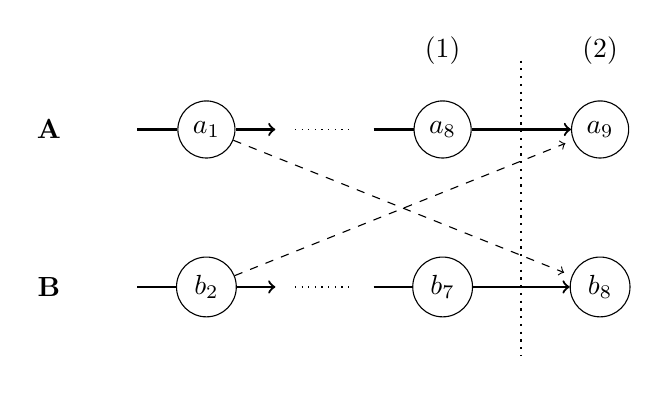
\begin{tikzpicture}
            \path
                node {\textbf{A}}
                to ++(0:1) node (a0) {}
                to ++(0:1) node[op] (a1) {$a_1$}
                to ++(0:1) node (a2) {}
                to ++(0:1) node (a7) {}
                to ++(0:1) node[op] (a8) {$a_8$}
                to ++(90:1) node {(1)}
                to ++(0:1) node (hideTop) {}
                to ++(270:1)
                to ++(0:1) node[op] (a9) {$a_9$}
                to ++(90:1) node {(2)};

            \draw[->, thick] (a0) --  (a1) -- (a2);
            \draw[dotted] (a2) -- (a7);
            \draw[->, thick] (a7) -- (a8) -- (a9);

            \path
                to ++(270:2) node {\textbf{B}}
                to ++(0:1) node (b0) {}
                to ++(0:1) node[op] (b2) {$b_2$}
                to ++(0:1) node (b3) {}
                to ++(0:1) node (b6) {}
                to ++(0:1) node[op] (b7) {$b_7$}
                to ++(0:1)
                to ++(270:1) node (hideBot) {}
                to ++(90:1)
                to ++(0:1) node[op] (b8) {$b_8$};

            \draw[->, thick] (b0) -- (b2) -- (b3);
            \draw[dotted] (b3) -- (b6);
            \draw[->, thick] (b6) -- (b7) -- (b8);

            \draw[->, dashed, shorten >= 3] (a1) -- (b8);
            \draw[->, dashed, shorten >= 3] (b2) -- (a9);

            \draw[dotted, thick] (hideTop) -- (hideBot);
        \end{tikzpicture}
        \caption{Execution}
        \label{fig:GC-execution}
    \end{subfigure}
    \begin{subfigure}{\columnwidth}
        \centering
        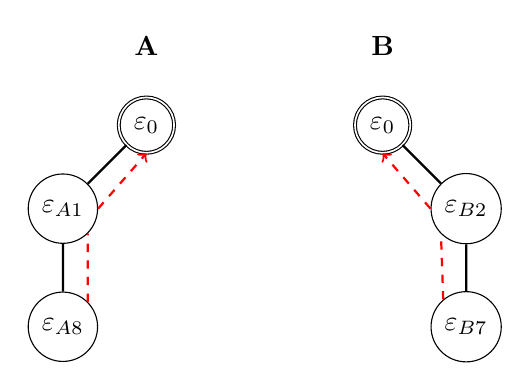
\begin{tikzpicture}
            \path
                node {\textbf{A}}
                to ++(270:1) node[causalop] (AeA0) {\epoch{0}}
                to ++(225:1.5) node[op] (AeA1) {\epoch{A1}}
                to ++(270:1.5) node[op] (AeA8) {\epoch{A8}};

            \path
                to ++(0:3) node {\textbf{B}}
                to ++(270:1) node[causalop] (BeB0) {\epoch{0}}
                to ++(315:1.5) node[op] (BeB2) {\epoch{B2}}
                to ++(270:1.5) node[op] (BeB7) {\epoch{B7}};


            \draw[thick] (AeA0) -- (AeA1) -- (AeA8);
            \draw[thick] (BeB0) -- (BeB2) -- (BeB7);
            \draw[->, dashed, thick, red] (AeA8.45) -- (AeA1.315) (AeA1.0) -- (AeA0.270);
            \draw[->, dashed, thick, red] (BeB7.130) -- (BeB2.225) (BeB2.180) -- (BeB0.270);

        \end{tikzpicture}
        \caption{States of respective epoch trees at (1)}
        \label{fig:GC-epoch-trees-step-1}
    \end{subfigure}
    \begin{subfigure}{\columnwidth}
        \centering
        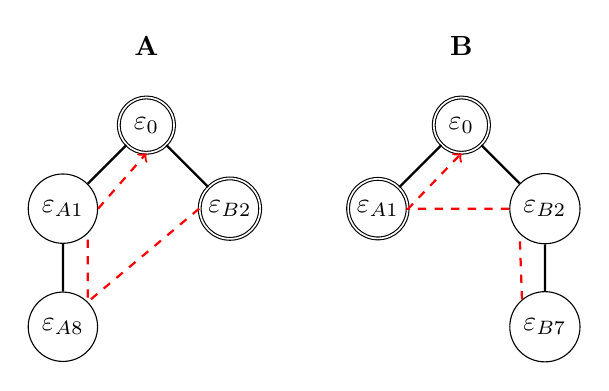
\begin{tikzpicture}
            \path
                node {\textbf{A}}
                to ++(270:1) node[causalop] (Ae0) {\epoch{0}}
                to ++(225:1.5) node[op] (AeA1) {\epoch{A1}}
                to ++(270:1.5) node[op] (AeA8) {\epoch{A8}};
            \path
                to ++(270:1)
                to ++(315:1.5) node[causalop] (AeB2) {\epoch{B2}};

            \path
                to ++(0:4) node {\textbf{B}}
                to ++(270:1) node[causalop] (Be0) {\epoch{0}}
                to ++(315:1.5) node[op] (BeB2) {\epoch{B2}}
                to ++(270:1.5) node[op] (BeB7) {\epoch{B7}};
            \path
                to ++(0:4)
                to ++(270:1)
                to ++(225:1.5) node[causalop] (BeA1) {\epoch{A1}};


            \draw[thick] (Ae0) -- (AeA1) -- (AeA8) (Ae0) -- (AeB2);
            \draw[thick] (Be0) -- (BeB2) -- (BeB7) (Be0) -- (BeA1);
            \draw[->, dashed, thick, red] (AeB2.180) -- (AeA8.45) -- (AeA1.315) (AeA1.0) -- (Ae0.270);
            \draw[->, dashed, thick, red] (BeB7.130) -- (BeB2.225) (BeB2.180) -- (BeA1.0) -- (Be0.270);

        \end{tikzpicture}
        \caption{States of respective epoch trees at (2)}
        \label{fig:GC-epoch-trees-step-2}
    \end{subfigure}
    \caption{Garbage collecting epochs and corresponding \emph{former states}}
    \label{fig:GC-epochs}
\end{figure}

\mnnote{TODO: Marquer comme GC \epoch{A1} et \epoch{A8} via \autoref{rule:gc-concurrent-primary-epoch} et \epoch{0} via \autoref{rule:gc-root} de l'epoch tree de A dans la \autoref{fig:GC-epoch-trees-step-2}}

\section{Evaluation}

\subsection{Simulations and benchmarks}

In order to validate the proposed approach, we proceed to an experimental evaluation.
The aims of this evaluation are to measure
\begin{enumerate*}[label=(\roman*)]
    \item the memory overhead of the replicated sequence
    \item the computational overhead added to \emph{insert} and \emph{remove} operations by the renaming mechanism
    \item the cost of integrating \emph{rename} operations.
\end{enumerate*}

Unfortunately, we were not able to retrieve an existing dataset of real-time collaborative editing sessions.
We thus setup simulations to generate the dataset on which run our benchmarks.
These simulations mimic the scenario below.

Several authors collaboratively write an article in real-time.
First of all, the authors mainly specify the content of the article.
Few \emph{remove} operations are issued in order to simulate spelling mistakes.
Once the document reaches a arbitrary given critical length, collaborators move on to the second phase of the simulation.
During this second phase, authors stop adding new content but instead focus on revamping existing parts.
This is simulated by balancing the ratio between \emph{insert} and \emph{remove} operations.
Every author has to issue a given number of \emph{insert} and \emph{remove} operations.
The simulation ends once every collaborators received all operations.
During the simulation, we take snapshots of the replicas' state at given steps to follow their evolution.

We ran simulations with the following experimental settings: we deployed 10 bots as separate Docker containers on a single workstation.
Each container corresponds to a single mono-threaded Node.js process simulating an author.
Bots share and edit collaboratively the document using either LogootSplit or RenamableLogootSplit according to the session.
In both cases, each bot performs an \emph{insert} or a \emph{remove} operation locally every 200 $\pm$ 50ms and broadcast it immediately to other nodes using a \ac{P2P} full mesh network.
During the first phase, the probabilities of issuing \emph{insert} and \emph{remove} operations are respectively of 80\% and 20\%.
Once the document reaches 60k characters (around 15 pages), bots switch to the second phase and set both probabilities to 50\%.
After each local operation, the bot may move its cursor to another random position in the document with a probability of 5\%.
Every bot generates 15k \emph{insert} or \emph{remove} operations and stops once it observed 150k operations.
Snapshots of the state of bot are taken periodically, every 10k observed operations.

Additionally, in the case of RenamableLogootSplit, from 1 to 4 bots are arbitrarily designated as \emph{renaming bots} according to the session.
\emph{Renaming bots} issue \emph{rename} operations every time they observe 30k operations overall.
These \emph{rename} operations are generated in a way ensuring that they are concurrent.

Code, benchmarks and results are available at: \url{https://github.com/coast-team/mute-bot-random/}.

\subsection{Results}

\paragraph{Convergence}

We first proceeded to verify the convergence of nodes states at the end of simulations.
For each simulation, we compared the final state of every nodes using their respective snapshots.
We were able to confirm that nodes eventually converged without any communication other than operations, thus satisfying the \ac{SEC} consistency model.

This result sets a first milestone in the validation of the correctness of RenamableLogootSplit.
It is however only empirical.
Further work to formally prove its correctness should be undertaken.

\paragraph{Memory overhead}

\begin{figure}[ht!]
    \centering
    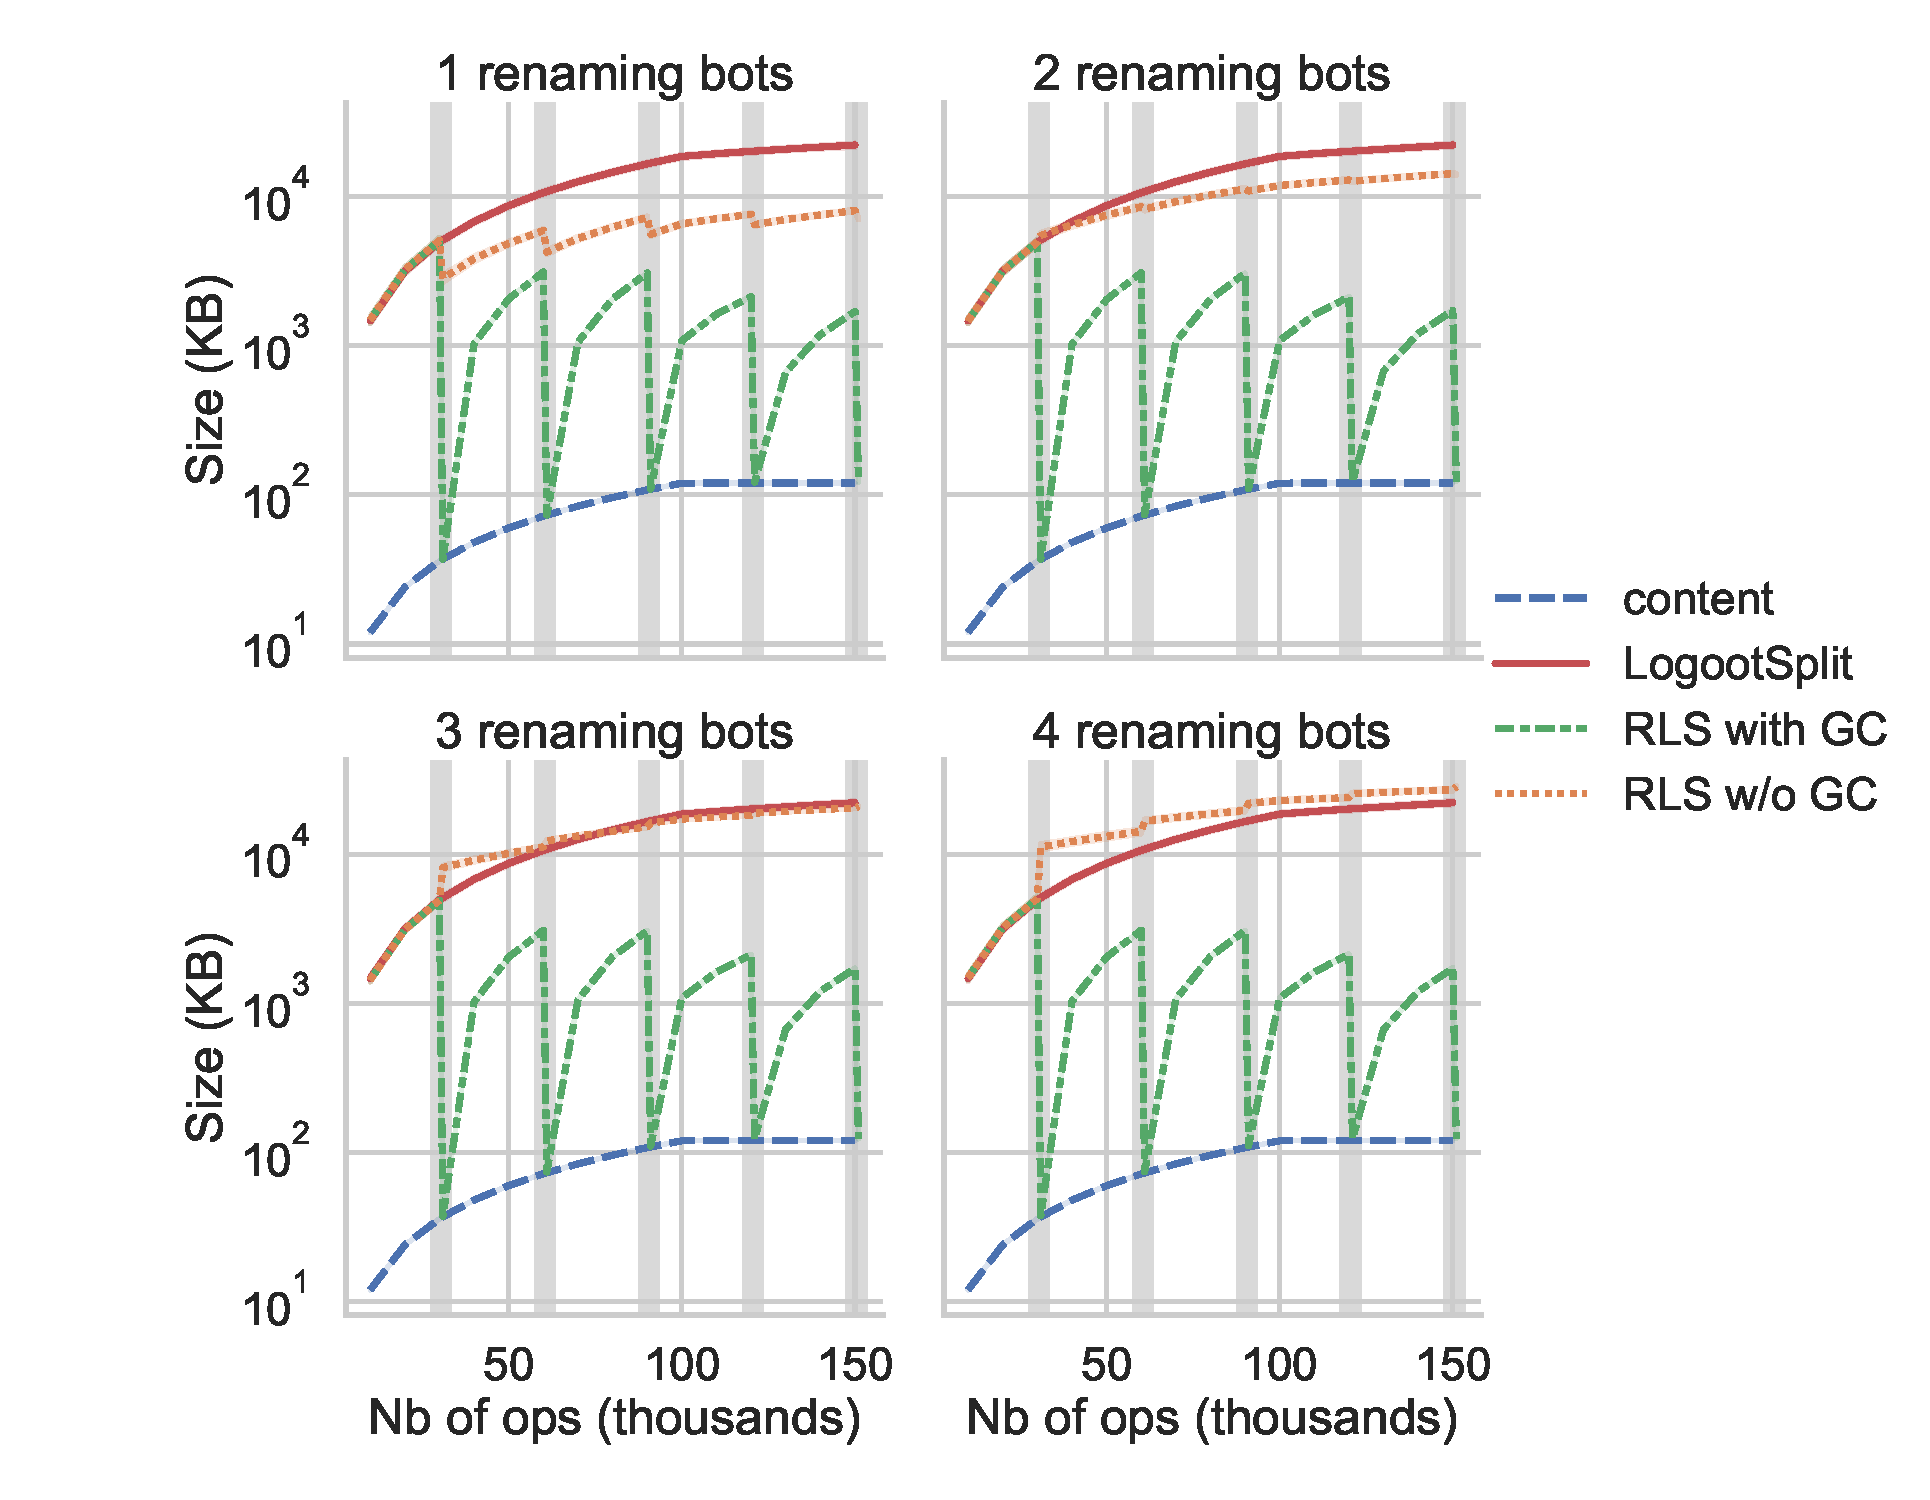
\includegraphics[width=\columnwidth]{img/snapshot-sizes.pdf}
    \caption{Evolution of the size of the document}
    \label{fig:evolution-document-size}
\end{figure}

We then proceeded to measure the evolution of the document's memory consumption throughout the simulations, according to the CRDT used and the number of \emph{renaming bots}.
We present the obtained results in \autoref{fig:evolution-document-size}.

For each plot displayed in \autoref{fig:evolution-document-size}, we represent 4 different data.
The blue dashed line illustrates the size of the actual content of the document, \ie the text, while the red line corresponds to the size of the whole LogootSplit document.

The green dashed-dotted line represents the size of the RenamableLogootSplit document in the best case scenario.
In this scenario, nodes assume that \emph{rename} operations are garbage-collectable as soon as they receive them.
Nodes are thus able to benefit the effects of the renaming mechanism while removing its own metadata, such as \emph{former states} and epochs.
In doing so, nodes are able to minimise periodically the metadata overhead of the data structure, independently of the number of \emph{renaming bots} and concurrent \emph{rename} operations issued.

On the other hand, the orange dotted line represents the size of the RenamableLogootSplit document in the worst case scenario.
In this scenario, nodes assume that \emph{rename} operations never become causally stable and can thus never be garbage-collected.
Nodes have to permanently store the metadata introduced by the renaming mechanism.
The performances of RenamableLogootSplit thus decrease as the number of \emph{renaming bots} and \emph{rename} operations issued increases.
Nonetheless, we observe that RenamableLogootSplit can outperform LogootSplit even in this worst case scenario while the number of \emph{renaming bots} remains low (1 or 2).
This result is explained by the fact that the renaming mechanism enables nodes to scrap the overhead of the internal data structure used to represent the document.

To summarise the results presented, the renaming mechanism introduces a temporary metadata overhead which increases with each \emph{rename} operations.
But the overhead will eventually subsides once the system becomes quiescent and \emph{rename} operations become causally stable.
In \autoref{sec:offloading-former-states}, we discuss that \emph{former states} may be offloaded until causal stability is achieved to address the temporary memory overhead.

\paragraph{Integration times of standard operations}

\begin{figure}[ht!]
    \begin{subfigure}{\columnwidth}
        \centering
        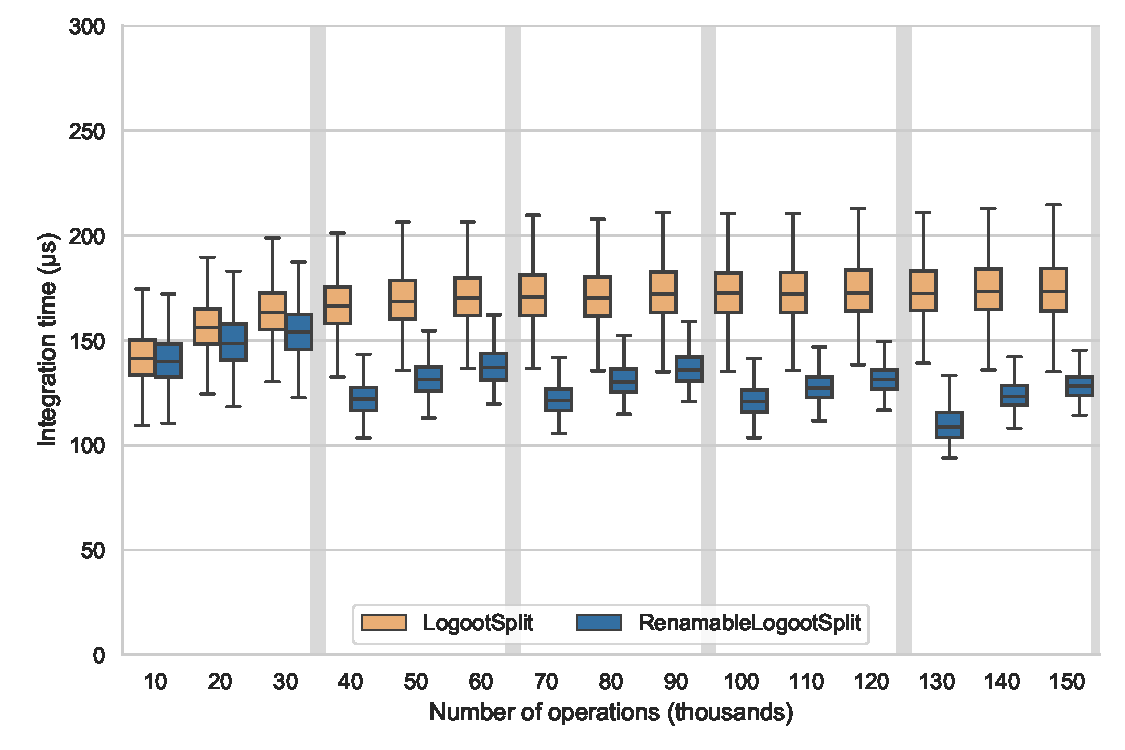
\includegraphics[width=0.9\columnwidth]{img/integration-time-boxplot-local-operations-without-outliers.pdf}
        \caption{Local operations}
        \label{fig:evolution-integration-time-local-insert}
    \end{subfigure}
    \begin{subfigure}{\columnwidth}
        \centering
        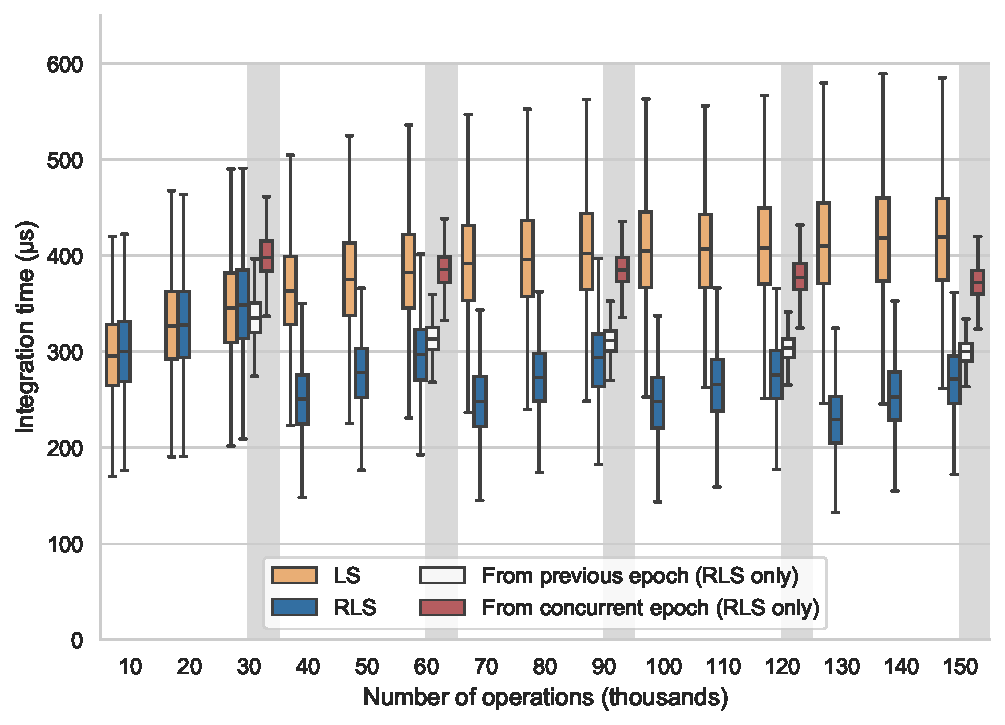
\includegraphics[width=0.9\columnwidth]{img/integration-time-boxplot-remote-operations-without-outliers.pdf}
        \caption{Remote operations}
        \label{fig:evolution-integration-time-remote-insert}
    \end{subfigure}
    \caption{Integration time of standard operations}
    \label{fig:evolution-integration-time-insert}
\end{figure}

We next compared the evolution of integration times of respectively local and remote operations on LogootSplit and RenamableLogootSplit documents.
\autoref{fig:evolution-integration-time-insert} displays obtained results.

In these figures, orange boxplots correspond to integration times on LogootSplit documents while blue ones correspond to times on RenamableLogootSplit documents.
While both are initially equivalent, integration times on RenamableLogootSplit documents are then reduced compared to LogootSplit ones once \emph{rename} operations have been applied.
This improvement is explained by the fact that \emph{rename} operations optimise the internal representation of the sequence.

Additionally, in the case of remote operations, we measured specific integration times for RenamableLogootSplit : integration times of remote operations from previous epochs and from concurrent epochs, respectively displayed as white and red boxplots in \autoref{fig:evolution-integration-time-remote-insert}.
Operations from previous epochs are operations generated concurrently to the \emph{rename} operation but applied after it.
Since the operation has to be transformed beforehand using \autoref{alg:renameId}, we observe a computational overhead compared to other operations.
But this overhead is actually compensated by the optimisation of the internal representation of the sequence performed by \emph{rename} operations.

Regarding operations from concurrent epochs, we observe an additional overhead as nodes have first to reverse the effect the concurrent \emph{rename} operation using \autoref{alg:revertRenameId}.
Because of this overhead, RenamableLogootSplit performances for these operations are comparable to LogootSplit ones.

To summarise, transformation functions introduce an overhead with regard to integration times of concurrent operations to \emph{rename} ones.
Despite this overhead, RenamableLogootSplit achieves better performances than LogootSplit as long as the distance between the epoch of generation of the operation and the current epoch of the node remains limited.
As the distance between both epochs increases, it leads to cases presenting worse performances than LogootSplit ones since the overhead is multiplied.
Nonetheless, the renaming mechanism reduces the integration times of the majority of operations, \ie the operations issued between two rounds of \emph{rename} operations.

\paragraph{Integration time of \emph{rename} operation}

\begin{figure}[ht!]
    \centering
    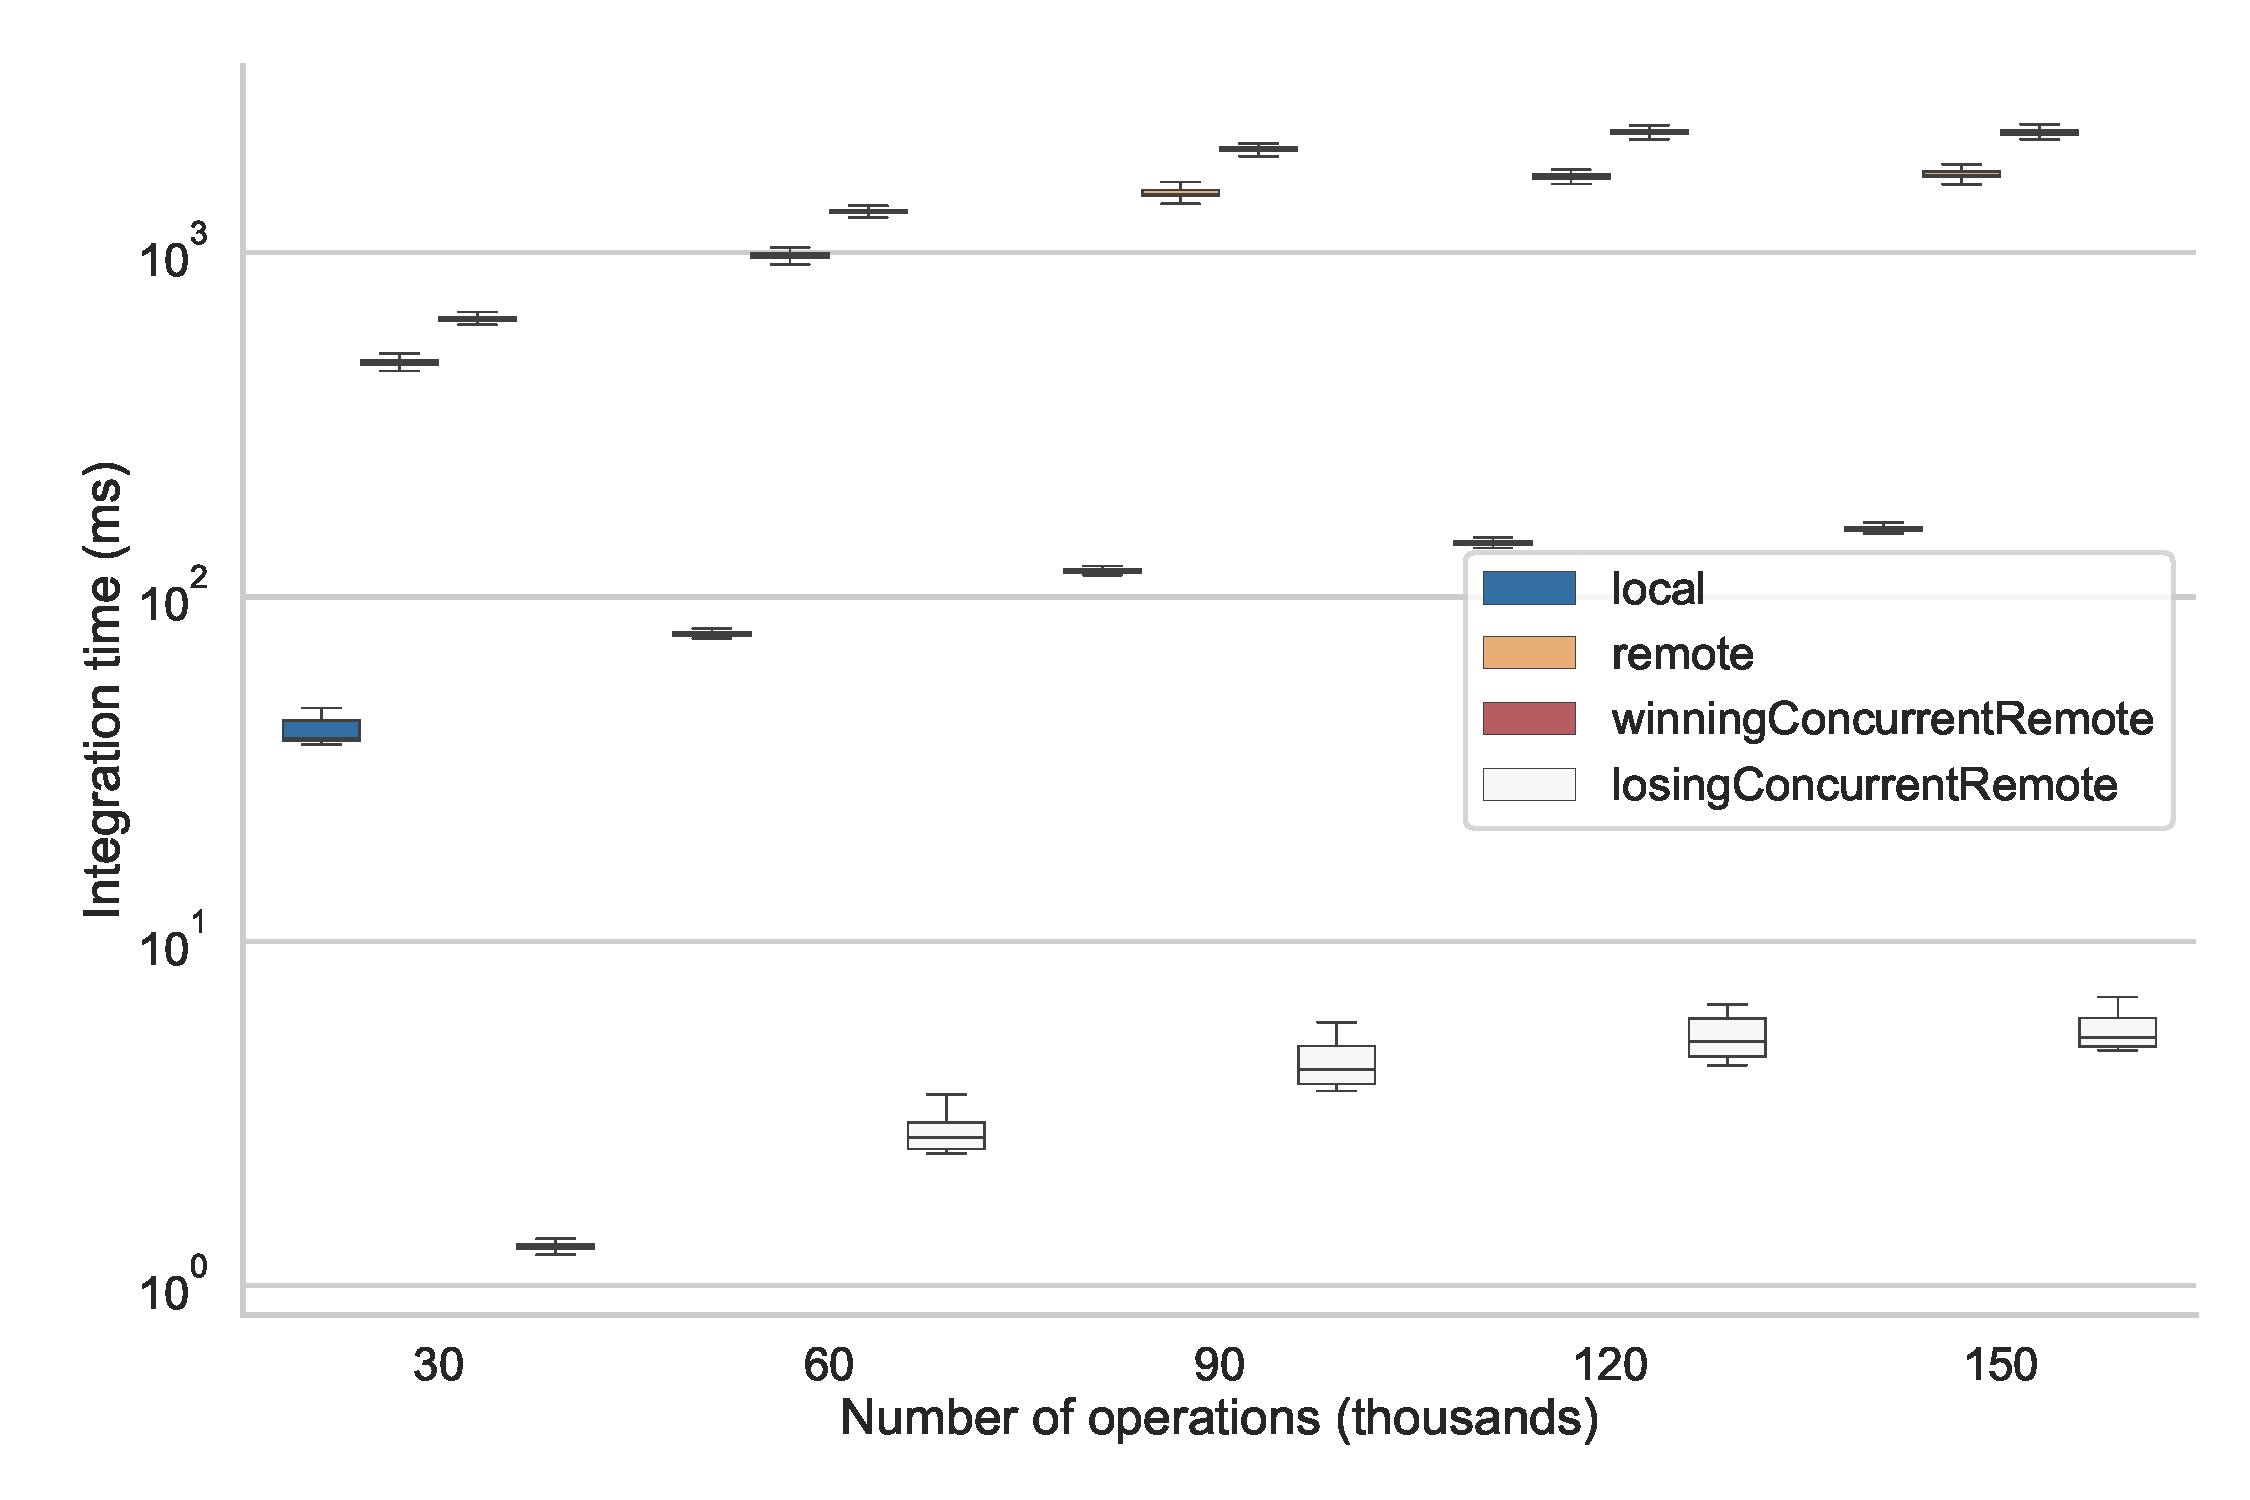
\includegraphics[width=\columnwidth]{img/integration-time-boxplot-rename-op-without-outliers.pdf}
    \caption{Integration time of rename operations}
    \label{fig:evolution-integration-time-rename}
\end{figure}

Finally, we measured the evolution of integration times of \emph{rename} operation according to the number of operations since the last \emph{rename} one.
The results are displayed in \autoref{fig:evolution-integration-time-rename}.

The main outcome of these measures are that \emph{rename} operations expensive compared to others.
Local \emph{rename} operations, represented here as blue boxplots, take hundreds of milliseconds while remote ones and concurrent \emph{primary} ones, respectively in orange and red, may last seconds if delayed for too long.
It is thus necessary to take this result into account when designing strategies to trigger \emph{rename} operations to prevent them from impacting negatively user experiences.

Another interesting result from this benchmark is that concurrent \emph{secondary rename} operations are cheap to apply, as they only consist in storing corresponding \emph{former states}.
Nodes can thus significantly reduce the overall computations of a set of concurrent \emph{rename} operations by applying them in a specific order.
We will discuss further this topic in \autoref{sec:postponing-transition-to-new-epoch}.

\section{Discussion}

\subsection{Offloading on disk unused \emph{former states}}
\label{sec:offloading-former-states}

As explained in \autoref{sec:reverting-rename-op}, nodes have to store \emph{former states} corresponding to \emph{rename} operations to transform operations from previous or concurrent epochs.
Nodes may receive such operations in 2 different cases :
\begin{enumerate*}[label=(\roman*)]
    \item nodes have recently issued \emph{rename} operations
    \item nodes logged back in the collaboration.
\end{enumerate*}
Between these specific events, \emph{former states} are actually not needed to handle operations.

We can thus propose the following trade-off : to offload \emph{former states} on the disk until their next use or that they can be garbage collected.
It would enable nodes to mitigate the temporary memory overhead introduced by the renaming mechanism but increases integration times of operations requiring one of these \emph{former states}.
Nodes could adopt various strategies to deem \emph{former states} offloadable and to retrieve them preemptively according to their constraints.
The design of these strategies could be based on several heuristics : epochs of currently online nodes, number of nodes still able to issue concurrent operations, time elapsed since last use of the \emph{former state}...

\subsection{Designing more effective \emph{priority} relation}
\label{sec:designing-more-effective-priority-relation}

Although the \emph{priority} relation proposed in \autoref{sec:priority} is simple and ensures that nodes designate the same epoch as the \emph{primary} one, it introduces a significant computational overhead in some cases.
Notably it allows a single node, disjoined from the collaboration since a long time, to force every other nodes to revert \emph{rename} operations they performed meanwhile because its own \emph{rename} operation is deemed as the \emph{primary} one.

The \emph{priority} relation should thus be designed to ensure convergence, but also to minimise the overall amount of computations performed by nodes of the system.
In order to design the \emph{priority} relation, we could embed into \emph{rename} operations metrics representing the state of the system and the accumulated work on the document (number of nodes currently at the \emph{parent} epoch, number of operations generated at the \emph{parent epoch}, length of the document...).
This way, we can favour the branch from the \emph{epoch tree} with the more and most active collaborators and prevent isolated nodes from overthrowing the existing order.

\subsection{Postponing transition to new epoch in case of high concurrency}
\label{sec:postponing-transition-to-new-epoch}

\begin{itemize}
    \item Primary remote \emph{rename} operations are expensive to integrate as nodes have to browse and rename their whole current state in the process
    \item It can introduce a significant computational overhead in some cases
    \item For example a node may receive concurrent \emph{rename} operations in the reverse order to the one set by the \emph{priority} relation
    \item The node would then consider each operation as the primary one and rename its state in a successive manner
    \item On the other hand, secondary remote \emph{rename} operations are cheap to integrate as nodes simply add to their state a reference to the corresponding \emph{former state}
    \item To reduce the likelihood and the negative impact of the scenario described previously, we can decompose the integration of \emph{rename} operations into two parts in case of concurrency detection
    \item Nodes first process \emph{rename} operations as secondary ones. It enables nodes to integrate remote \emph{insert} and \emph{remove} operations, even from concurrent epochs, by transforming them
    \item Then once nodes obtain a given amount of confidence that one \emph{rename} operation is the primary one, proceed to the renaming of their states
    \item This strategy introduces a slight overhead for each \emph{insert} or \emph{remove} operation received during this period, but reduces the probability of erroneously integrating \emph{rename} operations as primary ones
\end{itemize}

\section{Related work}

\subsection{The core-nebula approach}

\subsection{The LSEQ approach}

\section{Conclusions and future work}

\appendix

\section{Algorithms}

\begin{algorithm}
    \caption{Remaining functions to rename identifier}
    \begin{algorithmic}

    \Function{renIdFromIndex}{$\trm{pos}, \trm{nId}, \trm{nSeq}, \trm{index}$}
        \State \Return $\trm{new Id}(\trm{pos}, \trm{nId}, \trm{nSeq}, \trm{index})$
    \EndFunction
    \\
    \Function{renIdLessThanFirstId}{$\trm{id}, \trm{firstId}, \trm{newFirstId}$}
        \State $\trm{offset} \gets \trm{getLastOffset}(\trm{firstId}) - 1$
        \State $\trm{predOfFirstId} \gets \trm{createIdFromBase}(\trm{firstId}, \trm{offset})$
        \State $\trm{prefix} \gets \trm{concat}(\trm{predOfFirstId}, \trm{MAX\_TUPLE})$
        \State $\trm{predNewFirstId} \gets \trm{createIdFromBase}(\trm{newFirstId}, -1)$

        \If{$\trm{isPrefix}(\trm{prefix}, id)$}
            \State $\trm{tail} \gets \trm{getTail}(\trm{id}, \trm{prefix.length})$
            \State \Return $\trm{concat}(\trm{predNewFirstId}, \trm{tail})$
        \ElsIf{$\trm{id} < \trm{newFirstId}$}
            \State \Return $\trm{id}$
        \Else
            \State \Return $\trm{concat}(\trm{predNewFirstId}, \trm{id})$
        \EndIf
    \EndFunction
    \\
    \Function{renIdGreaterThanLastId}{$\trm{id}, \trm{lastId}, \trm{newLastId}$}
        \State $\trm{prefix} \gets \trm{concat}(\trm{lastId}, \trm{MIN\_TUPLE})$

        \If{$\trm{isPrefix}(\trm{prefix}, id)$}
            \State $\trm{tail} \gets \trm{getTail}(\trm{id}, \trm{prefix.length})$
            \State \Return $\trm{tail}$
        \ElsIf{$\trm{newLastId} < \trm{id}$}
            \State \Return $\trm{id}$
        \Else
            \State \LeftComment{$\trm{lastId} < \trm{id} < \trm{newLastId}$}
            \State \Return $\trm{concat}(\trm{newLastId}, \trm{id})$
        \EndIf
    \EndFunction
    \end{algorithmic}
\end{algorithm}

\begin{algorithm}
    \caption{Remaining functions to revert identifier renaming}
    \begin{algorithmic}

    \Function{revRenIdLessThanNewFirstId}{$\trm{id}, \trm{firstId}, \trm{newFirstId}$}
        \State $\trm{predNewFirstId} \gets \trm{createIdFromBase}(\trm{newFirstId}, -1)$
        \If{$\trm{predNewFirstId} < \trm{id}$}
            \State $\trm{tail} \gets \trm{getTail}(\trm{id}, 1)$
            \If{$\trm{tail} < \trm{firstId}$}
                \State \Return $\trm{tail}$
            \Else
                \State $\trm{offset} \gets \trm{getLastOffset}(\trm{firstId})$
                \State $\trm{predFirstId} \gets \trm{createIdFromBase}(\trm{firstId}, \trm{offset}) $
                \State \Return $\trm{concat}(\trm{predFirstId}, \trm{MAX\_TUPLE}, \trm{tail})$
            \EndIf
        \Else
            \State \Return $\trm{id}$
        \EndIf
    \EndFunction
    \\
    \Function{revRenIdGreaterThanNewLastId}{$\trm{id}, \trm{lastId}$}
        \If{$\trm{id} < \trm{lastId}$}
            \State \Return $\trm{concat}(\trm{lastId}, \trm{MIN\_TUPLE}, \trm{id})$
        \Else
            \State \Return $\trm{id}$
        \EndIf
    \EndFunction
    \end{algorithmic}
\end{algorithm}

\bibliography{ref}

\end{document}
